\section{Stability study}
An unavoidable issue with the explicit time integration of the velocity-Verlet algorithm is stability. In this section we find stable DEM timesteps as a function of material properties of ceramic pebbles. With that knowledge in hand, we argue for scaling certain physical properties to allow for faster simulations.

\subsection{Critical timestep}

\begin{align}
\delta t_c = \eta  \sqrt{\frac{m_0}{k_0}}
\end{align}
where $m_0$ is the smallest particle mass, related to the smallest particle radius, $R_0$. The value of $\eta$ is less than unity and depends on the integration algorithm as well as dimensions of freedom [site O'Sullivan].
\begin{align}
m_0 = \frac{4}{3} \pi R_0^3 \rho
\end{align}
and we assume all pebbles have the same density, $\rho$. $k_0$ is the maximum normal stiffness in the ensemble. The timestep chosen for the DEM must be less than this critical timestep.
\begin{align}
\Delta t \le \delta t_c
\end{align}

From Hertz theory, the maximum normal contact stiffness is
\begin{align}
k_0 = \frac{4}{3} E^* \sqrt{R^*_0 \delta_0}
\end{align}

To find the maximum contact stiffness (neglecting the influence of $\delta_0$ for the moment), we will express the relative radius in an alternate form,
\begin{align}
\frac{1}{R^*_0} = \frac{1}{R_0} + \frac{1}{\gamma R_0}
\end{align}
where $\gamma \ge 1$, it is a parameter that indicates our smallest pebble of radius $R_0$ is interacting with another pebble that is either the same size or larger. In the limits, if $\gamma =1$, then $R^*_0 = \frac{R_0}{2}$. If $\gamma \rightarrow \infty$, then $R^*_0 = R_0$. The stiffness is positively proportional to relative radius. Therefore if we desire the maximum contact stiffness, we need the largest value of $R^*_0$ and thus require $\gamma \rightarrow \infty$.

With $R^*_0 = R_0$, we use this in the formula for pebble mass term of the stability criteria 
\begin{align}
\delta t_c &= \eta  \sqrt{\frac{\frac{4}{3} \pi (R^*_0)^3 \rho}{\frac{4}{3} E^* \sqrt{R^*_0 \delta_0}}}\\
\delta t_c &= \left[ \eta \sqrt{ \pi} \right] \rho^{1/2}\left(\frac{1}{E^*}\right)^{1/2} \left(\frac{1}{\delta_0}\right)^{1/4}(R^*_0)^{5/4}
\end{align}

We can relate the maximum pebble overlap $\delta_0$ to the maximum contact force in the ensemble with Eq.~\ref{eq:hertzForce}, after some algebra we find
\begin{align}
\delta t_c &= \left[ \eta \sqrt{ \pi} (4/3)^{1/6} \right] \rho^{1/2} \left(\frac{1}{F_\text{max}}\right)^{1/6} \left(\frac{1}{E^*}\right)^{1/3} R^{*5/4}_0
\end{align}

The term in the bracket is a constant near unity. Neglecting it, we see the timestep is proportional to these terms,
\begin{align}\label{eq:stability-terms}
\delta t_c \propto \rho^{1/2} \left(\frac{1}{F_\text{max}}\right)^{1/6} \left(\frac{1}{E^*}\right)^{1/3} R^{*5/4}_0
\end{align}

Figure~\ref{fig:stability-curves} provides visual reinforcement of the powers of terms in Eq.~\ref{eq:stability-terms}; it is the impact of different normal-contact parameters on the stable timestep. 
\begin{figure}[ht!]
\centering
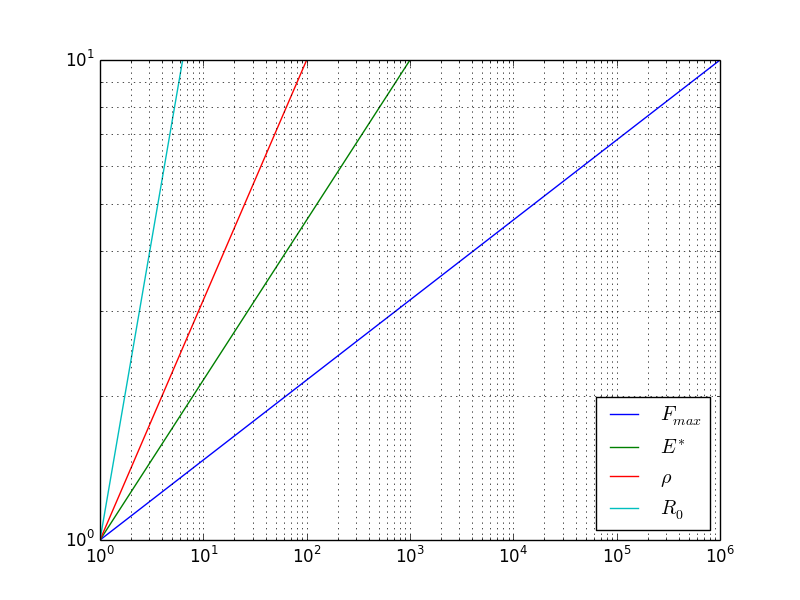
\includegraphics[width = 0.75 \textwidth]{chapters/figures/stability_curves}
\caption{Curves showing the rate of response to timestep on the various normal-contact parameters.}\label{fig:stability-curves}
\end{figure}

It is apparent that simulations become less stable primarily as the pebble diameter decreases and then slightly less so for decreasing density and increasing the effective Young's modulus. It takes a rather large increase in the maximum contact force to cause the stable timestep to decrease. This is a fortunate result as it is primarily material properties which dictate stability of a DEM simulation. If external pressures increase and cause increases in the maximum normal contact force in the ensemble, it is unlikely to cause instabilities in the model. The result also provides insight into scaling of physical parameters to allow larger timesteps and thereby shorter overall duration of simulations.

The ceramic materials identified for breeders have relatively high Young's moduli, on the order of \si{10^{10} Pa}. The smallest radius will be on the order of \si{10^{-4} m}. The ceramic density is approximately on the scale of \si{10^{4} kg/m^3}. Finally, to prevent pebbles from cracking in the ensemble, it is reasonable to assume that the maximum contact forces will on the order of \si{10^2 N}. These values lead to a necessary timestep of
\begin{align}
\delta t_c \propto 10^{-7} \si{s}
\end{align}



\subsection{Simulation acceleration with scaled material properties}
As we saw with Eq.~\ref{eq:stability-terms}, if we wish to increase the timestep of our DEM simulations, we would be rewarded more quickly if scaling, for example, the material density rather than Young's modulus.


